\subsubsection{Hydrological Water Balance}
To characterize the field-scale water balance we use a simple single-layer model of soil moisture at a point. The overall water balance is given by:

\begin{equation}
\label{eq:h2o}
    n Z_r \frac{\text{d}s(t)}{\text{d}t} = R(t) - ET(s(t)) - L(s(t)) - Q(s(t)),
\end{equation}

\noindent
where $n$ is porosity [-], $Z_{\text{r}}$ is the rooting depth [mm], $s(t)$ is the saturation, or relative soil moisture content ($0 \leq s(t) \leq 1$), $R(t)$ is the rainfall rate [mm day$^{-1}$], $E(s(t))$ is the rate of evapotranspiration [mm day$^{-1}$], $L(s(t))$ is the rate of leakage [mm day$^{-1}$], and $Q(s(t),t)$ is the runoff rate [mm day$^{-1}$]. This is analogous to Eq. 1 from Rodriguez-Iturbe, et al. (2001), with the rate of interception by the canopy taken to be 0. 

In maize systems, rainfall interception by the canopy will be highest during tasseling (reproductive) and maturity stages \cite{zheng2018rainfall}. The degree to which rainfall is intercepted depends on a number of factors that can be site and canopy-specific. For instance, recent field studies in China, Iran and Indonesia indicate that canopy partitioning varies greatly and results are site-specific \cite{van2001modelling, zheng2018rainfall, nazari2020rainfall}. Because there are no field studies of rainfall interception by maize in Kenya (only studies that investigate the role of intercropping \textit{Grevillea robusta} with maize, e.g. \citeA{ong2000productivity, jackson2000measured}), we chose not to include interception in the model.

\paragraph{Rainfall}

Rainfall is treated as a non-stationary marked Poisson process. In each dekad (10-day increment) $i$, rainfall occurs with a probability, $\lambda_i$ [day$^{-1}$], and the depth of rainfall events are drawn from an exponential distribution with a mean value, $\alpha_i$ [mm]. Average dekadal values of $\lambda$ and $\alpha$ are estimated from a long-term rainfall record of daily station rainfall data, which was described previously in section \ref{historic-rainfall}. Using a fixed average $\lambda_i$ value for each dekad underestimates the variance in seasonal rainfall and does not accurately represent the observed coefficient of variation in seasonal rainfall for this region. Therefore, we allow dekadal $\lambda_i$ values to vary for each season by scaling all $\lambda_i$ values by a random, season-specific scale factor drawn from a normal distribution with a mean of 1 and a standard deviation of 0.35. This allows us to capture the coefficient of variation of seasonal rainfall at the Ol Jogi and Jacobson Farm stations. 

% Previously in this section but removed:
 %. with the probability density function

% \begin{equation}
% \label{eq:alpha}
%     f_{X,i}(x) = \frac{1}{\alpha_i} \mathrm{e}^{-\frac{x}{\alpha_i}}.
% \end{equation}

% This is repetitive I think
% We fit daily rainfall volumes from a long-term rainfall data set with 30+ years of data to an exponential distribution and return a fitted PDF for a given rainfall climatology (i.e. rain gauge). We test the fit of our exponential distribution with an empirical histogram to check that the modeled rainfall has a r-squared value above 0.9. To simulate daily rainfall values, we generate a time series of rainfall based on the parameters $\lambda$ and $\alpha$. To calculate an alpha value per month we find all of the daily rainfall values where rain was greater than 0 and fit the daily rainfall amounts to an exponential distribution to get a monthly alpha value. Then we calculate the monthly lambda value by dividing the number of rainy days by the total number of days in a month. Then to simulate daily rainfall values, we generate a time series of rainfall based on the parameters alpha and lambda and or the length of season. 

\paragraph{Evapotranspiration}

Evapotranspiration depends on both the soil moisture, $s$, and the time into the growing season, $t$. We separate evapotranspiration into its two components, soil evaporation $E(s,t)$ and plant transpiration $T(s,t)$ such that
\begin{equation}
\label{eq:ET1}
    ET(s,t) = E(s,t) + T(s,t).
\end{equation}

\noindent
Soil evaporation depends on both the amount of soil moisture and the extent of the crop canopy, which intercepts radiation and reduces energy available for soil evaporation. We define Evaporation as 

\begin{equation}
\label{eq:E}
    E(s,t) = \begin{cases}
        0   &   0 \leq s < s_{\text{h}}  \\
        \left( \frac{s-s_{\text{h}}}{1-s_{\text{h}}} \right) ^{q_{\text{e}}} ET_{\text{max}} \mathrm{e}^{-0.5 \cdot LAI(t)}  &   s_{\text{h}} \leq s \leq 1 \\
    \end{cases},
\end{equation}

\noindent
where $q_{\text{e}}$ represents the non-linear rate at which soil evaporation declines as soil moisture drops below saturation, $LAI$ denotes the crop leaf area index [mm$^2$ mm$^{-2}$], a measure of canopy density, and $s_{\text{h}}$ is the soil moisture at the hygroscopic point. $LAI(t)$ varies depending on the time into the growing season, $t$, and is calculated from the maximum leaf area index of a given crop, $LAI_{c,max}$ and the crop coefficient, $K_c(t)$, as follows:

\begin{equation}
\label{eq:lai}
    LAI(t) = LAI_{\text{c,\text{max}}} \frac{K_c(t)}{K_{c, \text{max}}}
\end{equation}

\noindent

\paragraph{Seasonal variation in the Crop coefficient}
The growing season is divided into four stages of crop phenology, through which the crop coefficient varies, peaking in mid-season after the reproductive stage. The crop coefficient is determined as

\begin{equation}
\label{eq:Kc}
    K_c(t) = \begin{cases}
        K_{c,\text{ini}}
            &   t \leq f_\text{i} \\[6pt]
            
        \frac{K_{c,\text{max}}-K_{c,\text{ini}}}{f_\text{d} - f_\text{i}} (t- f_\text{i}) + K_{c,\text{ini}}
            &   f_\text{i} < t \leq f_\text{d}   \\[6pt]
            
        K_{c,\text{max}}
            &   f_\text{d}  < t \leq f_\text{ms}   \\[6pt]
            
        \frac{K_{c, \text{eos}}-K_{c,\text{max}}} {f_\text{ls} - f_\text{ms}}  (t- f_\text{ms}) + K_{c,\text{max}}
            &   f_\text{ms} < t < f_\text{ls}  \\[6pt]

        K_{c,\text{eos}}
            &   t = f_\text{ls}
    \end{cases}
\end{equation}

\noindent
where $f_\text{i}$, $f_\text{d}$, $f_\text{ms}$, and $f_{\text{ls}}$ denote the time in days from the beginning of the growing season to the vegetative period (initial), reproductive period (development), maturity period (mid-season), and end of season (late season), respectively. The values of $K_c$ during vegetative and ripening periods are constant functions of time and the values of $K_c$ during reproductive and senescence stages are linearly interpolated between the values for the start and end of each period. We use crop coefficient ($K_c$) values based on those listed in FAO guidelines for 180-day maize (grain) in high altitude East Africa, which are defined as 0.3, 0.3, 1.2, 1.2, and 0.6 and correspond to 0\%, 16\%, 44\%, 76\% and 100\% of the growing season \cite{allen1998chapter}. We selected this metric for $K_c$ because it is widely used in the Crop Water Requirement Satisfaction Index (WRSI) \cite{senay2004crop} when locally appropriate values are absent. % the initial, mid-season, and end of season, respectively. 
%\citeA{allen1998chapter} provides crop development stages for a 180-day variety, which we use in our calculation of crop coefficient: $L_{\text{ini}=30}$, $L_{\text{dev}}$ = 50, $L_{\text{mid}}$ = 60, $L_{\text{late}}$ = 40. 

The rate of plant transpiration, $T(s)$, is given as

\begin{equation}
\label{eq:T}
    T(s) = \begin{cases}
        0   &   s < s_{\text{w}}  \\
        \frac{s - s_{\text{w}}}{s^* - s_{\text{w}}} K_c T_{\text{max}}    &   s_{\text{w}} \leq s < s^*  \\
        K_c T_{\text{max}}  &   s^* \leq s \leq 1 \\
    \end{cases}
\end{equation}

\noindent
where $T_{\text{max}}$ is the maximum transpiration rate of the plant, $s_{\text{w}}$ is the soil moisture at the wilting point, and, $s^{*}$ is the soil moisture at the stress point.

Having solved for the components of Eq.~\ref{eq:ET1}, we can use Eqs.~\ref{eq:E} and ~\ref{eq:T} express $ET(s)$ as follows:

\begin{equation}
\label{eq:ET2}
    ET(s) = \begin{cases}
    0   &   0 \leq s < s_{\text{h}}   \\[6pt]
    \left( \frac{s-s_{\text{h}}}{1-s_{\text{h}}} \right) ^{q_{\text{e}}} ET_{\text{max}} \mathrm{e}^{-0.5 \cdot LAI} 
        &   s_{\text{h}} \leq s < s_{\text{w}}   \\[6pt]

    \left( \frac{s-s_{\text{h}}}{1-s_{\text{h}}} \right) ^{q_{\text{e}}} ET_{\text{max}} \mathrm{e}^{-0.5 \cdot LAI} + \frac{s - s_{\text{w}}}{s^* - s_{\text{w}}} K_c T_{\text{max}} 
        &   s_{\text{w}} \leq s < s^*   \\[6pt]
    \left( \frac{s-s_{\text{h}}}{1-s_{\text{h}}} \right) ^{q_{\text{e}}} ET_{\text{max}} \mathrm{e}^{-0.5 \cdot LAI} + 
    K_c T_{\text{max}}
        &   s^* \leq s \leq 1  
    \end{cases}
\end{equation}

Figure \ref{fig:et} shows the functional form of evaporation and transpiration as a function of relative soil moisture content for a clay loam soil in which $s_{\text{h}}$ is 0.42, $s_{\text{w}}$ is 0.53, and $s^{*}$ is 0.78.

\begin{figure}%[ht]
\centering
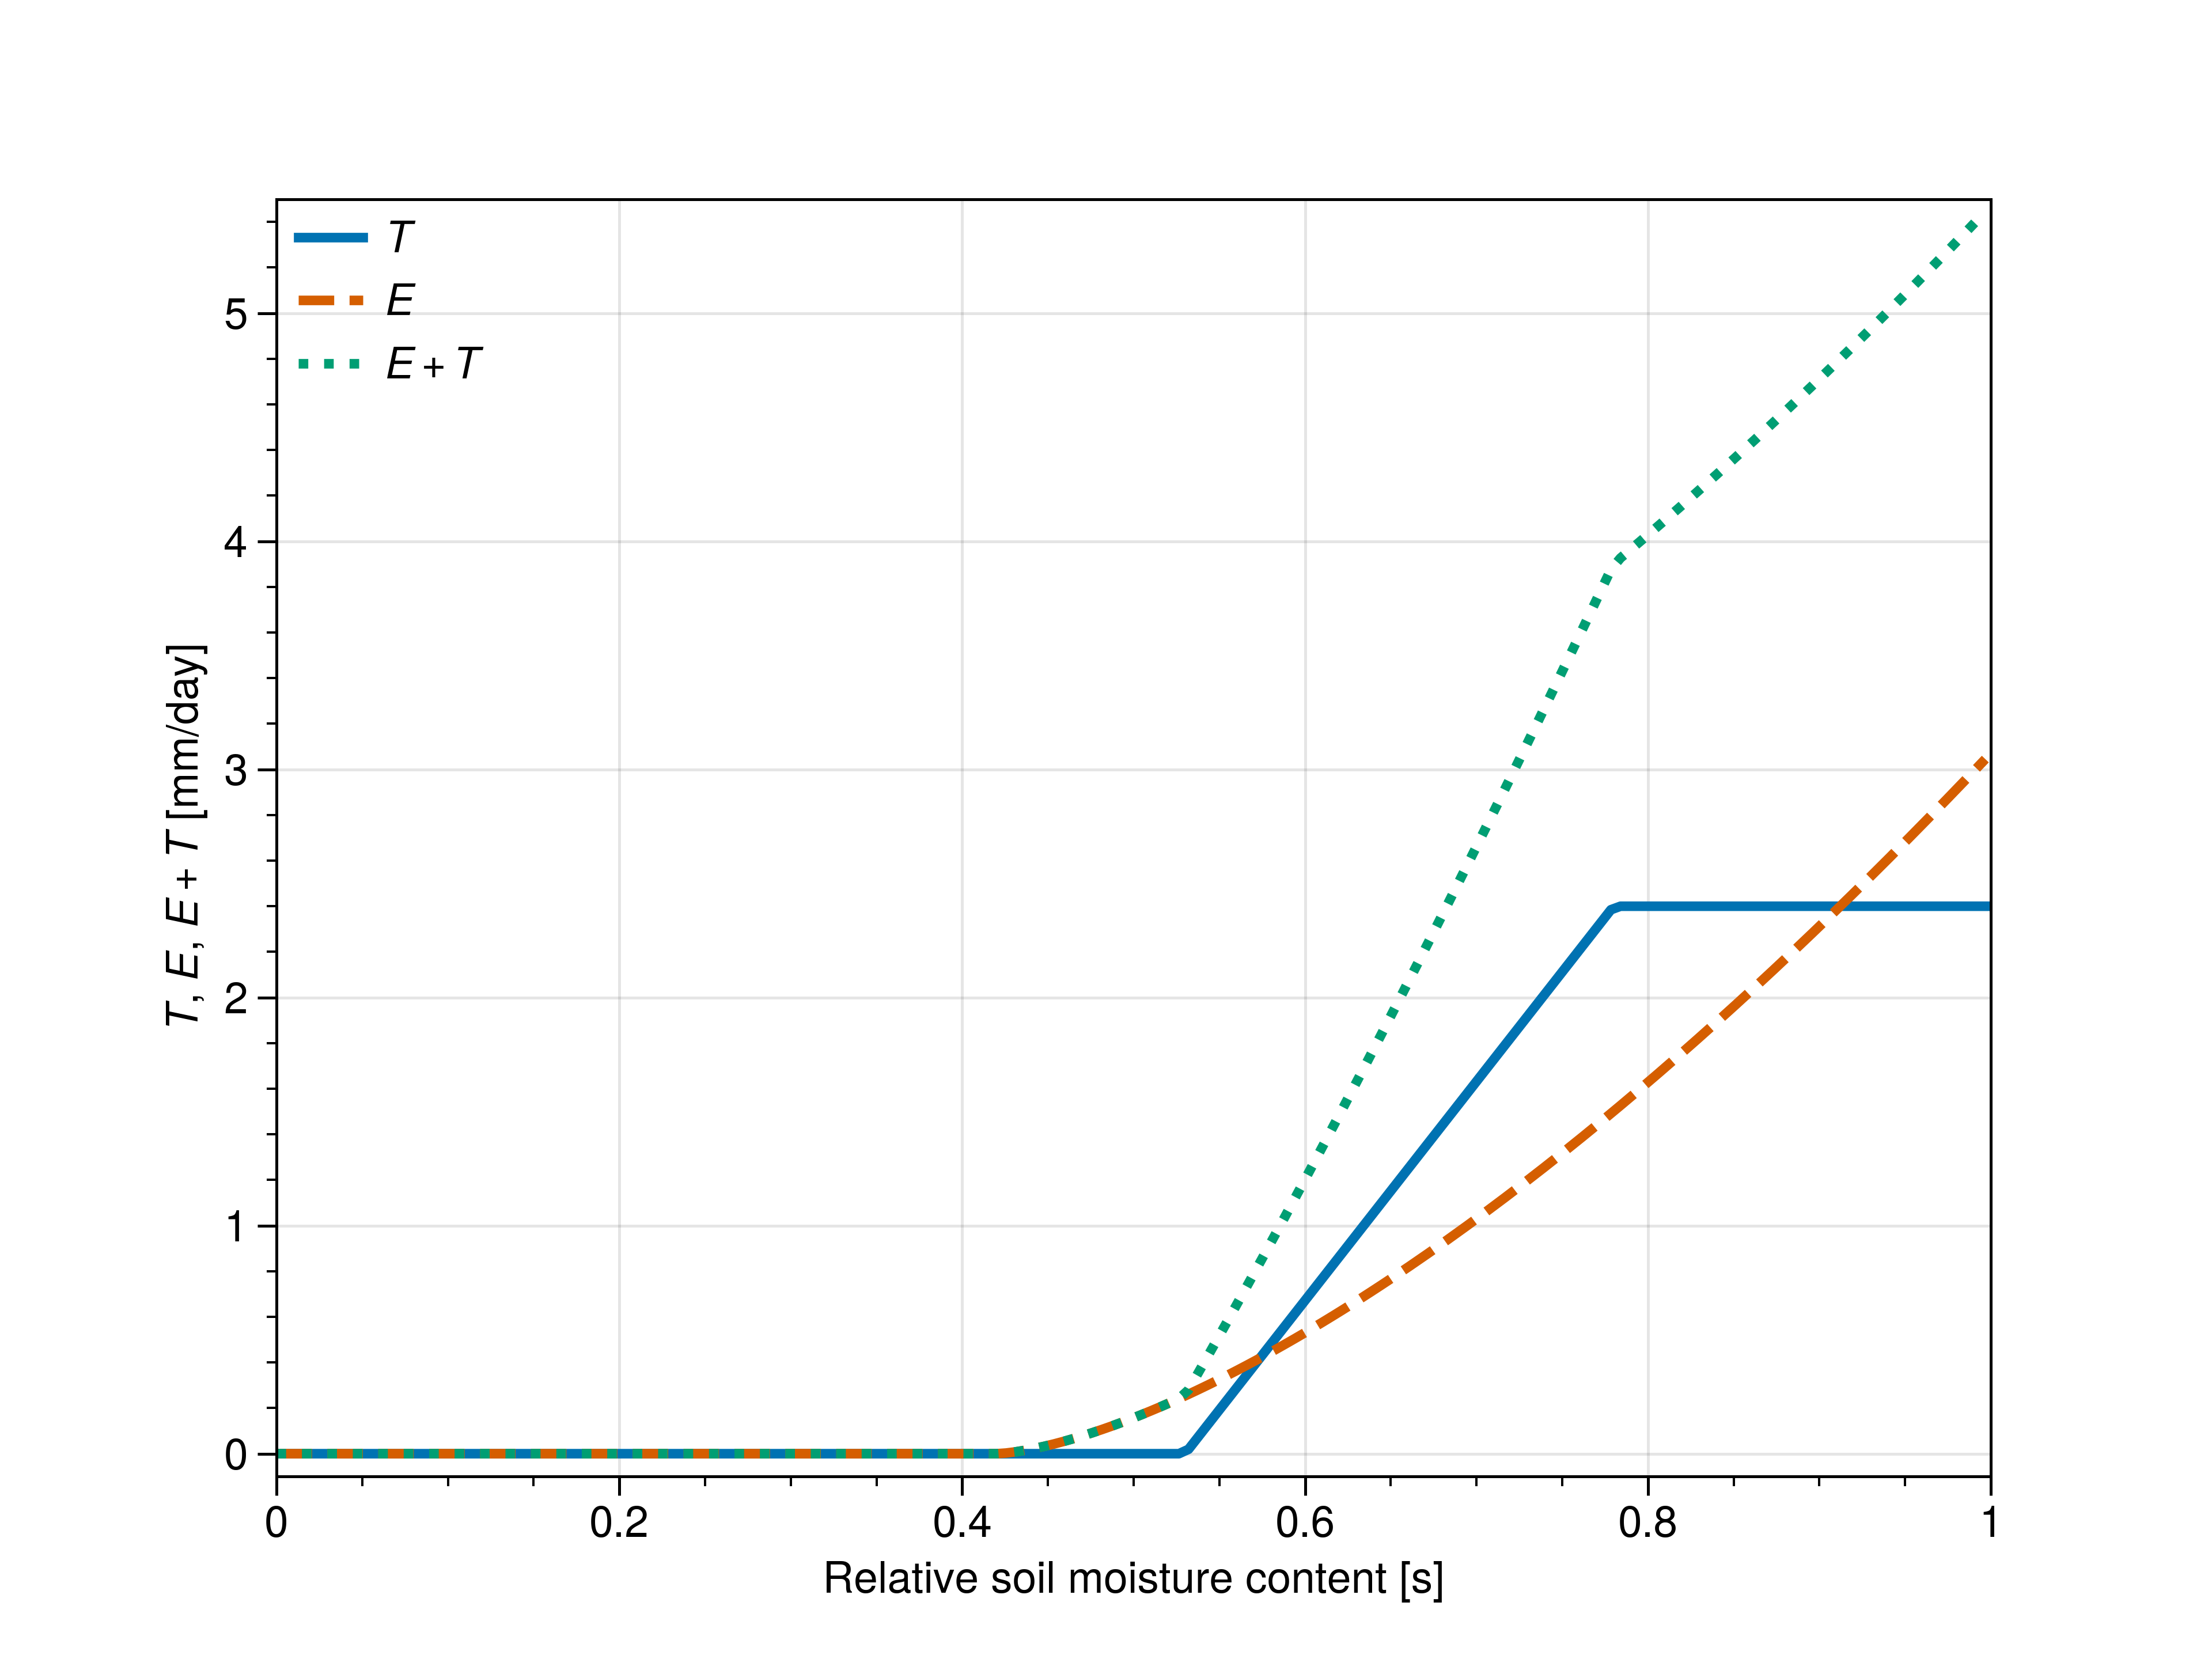
\includegraphics[width=100mm]{fig4_ET.png}
\caption{Evaporation, transpiration, and evapotranspiration as functions of relative soil moisture where LAI is 1.5 and $s_{\text{h}}$ is 0.42. Other climate and crop parameters are those listed in Table \ref{table:parameters}. }
\label{fig:et}
\end{figure}


\paragraph{Leakage}

Whenever daily soil moisture exceeds the soil field capacity, $s_{fc}$, we calculate leakage of water out of the plant root zone. The instantaneous rate of leakage is determined by the hydraulic conductivity, K(s) [mm/day], which is given by

\begin{equation}
\label{eq:K_s}
    L(s) = K(s) = \frac{K_s} {\mathrm{e}^{\beta(1-s_{\text{fc}})}-1} (\mathrm{e}^{\beta(s-s_{\text{fc}})}-1),
\end{equation}

\noindent
where $K_s$ is the saturated hydraulic conductivity [mm/day] and $\beta$ is a soil-specific parameter that governs the shape of the relationship between saturation and hydraulic conductivity; that is, $\beta = 2b + 4$, where $b$ is a  coefficient governing the power-law form of the soil-water retention curve \cite{Laio2001-fe}. 

\begin{equation}
    \varPsi_s = \overline{\varPsi}_s \, s^{-b}
\end{equation}

\noindent
where $\varPsi_s$ is the soil matrix potential at a given value of soil moisture and $\overline{\varPsi}_s$ is the geometric mean of the soil matrix potential values in the curve. Values of $b$ are based on soil texture and are taken from the empirically-determined coefficients presented in \citeA{clapp1978empirical}. 

Following an input of rainfall such that $s_0 >  s_{\text{fc}}$, Eq.~\ref{eq:h2o} becomes an expression of soil moisture decay. In the absence of evaporative losses, we can simplify leakage to

\begin{equation}
\label{eq:loss}
    L(s) = - n Z_{\text{r}} \frac{\text{d}s} {\text{d}t} 
\end{equation}

Then we use Eqs.~ \ref{eq:K_s} and \ref{eq:loss} to solve for the initial condition, $s_0$, which yields the solution for total daily leakage when $s >  s_{\text{fc}}$: 

\begin{equation}
\label{eq:L}
    L= \frac{n Z_{\text{r}}}{\beta} \ln{\left[ \mathrm{e}^{\beta (s_0 - s_{\text{fc}})} - \mathrm{e}^{-m \beta} (\mathrm{e}^{\beta (s_0 - s_{\text{fc}})} - 1 ) \right] }
\end{equation}

where 

\begin{equation}
\label{eq:m}
    m = \frac{K_s}{n Z_{\text{r}} \left( \mathrm{e}^{\beta (1 - s_{\text{fc}})} - 1 \right)}
\end{equation}


\paragraph{Runoff}

Our model only considers saturation excess overland flow, so that when the balance of daily rainfall, evaporation, and leakage leads to an excess of soil saturation, the excess is converted to surface runoff. Thus, we can write

\begin{equation}
\label{eq:Q}
    Q(s) = \begin{cases}
        0           &   0 \leq s \leq 1 \\
        (s-1) n Z_{\text{r}}  &   s > 1
    \end{cases}
\end{equation}


\vskip 24pt


\subsubsection{Plant Water Stress}

Water stress during the growing season affects the physiology of plants and is crucial in determining the success of a crop. Soil moisture excursions below the wilting point, $s_w$, and the point at which transpiration is reduced, $s^{*}$, can lead to reduced biomass production and eventual crop failure. By defining the duration and frequency of soil moisture deficits probabilistically, we gain insight into the yield reductions from intense water stress such as drought and the likelihood of crop failure. The mathematical derivations for these dynamics are described in previous work (e.g. \citeA{rodriguez2007ecohydrology}.)

First we calculate static water stress: a measure of the mean vegetation water stress stress incurred during a given excursion below $s^{*}$ \cite{Porporato2001-ui}.

\begin{equation}
\zeta(t) = \left[ \frac{s^*-s(t)}{s^*-s_w} \right]^{q_{\text{stress}}}\text{,        for } s_w \leq s(t) \leq s^*
\end{equation}

where $\zeta(t)$ is the static water stress and $q_{\text{stress}}$ represents the crop's sensitivity to the magnitude of excursions below the stress point.

Although the static stress describes the mean water deficit relative to $s^*$ and $s_w$, we are also interested in the duration and frequency of water deficit. Following the work of \citeA[p.~67]{rodriguez2007ecohydrology}, we also define two other random variables: the average length of time in days in which soil moisture is below the threshold, $T_\zeta$, and the number of times the threshold is crossed during a season, $n_\zeta$. Next, we calculate dynamic water stress, $\theta$, a measure of the crop's total water stress during the growing season that characterizes the duration and frequency of exposure to water stress:

\begin{equation}
    \theta = \begin{cases}
        \left( \frac{{\overline{\zeta} \, } \overline{{{T}}_{s*}}}{k{LGP}} \right)^{n^{-r}_{s^*}}
        &\text{,    }   \overline{\zeta} \, \overline{{T}_{s*}} < k{LGP} \\
        
        1  & \text{, }    {\overline{\zeta} \, } \overline{{{T}}_{s*}} \geq k{LGP}
    \end{cases}
\end{equation}

% \theta = \left( \frac{{\overline{\zeta} \, } \overline{{{T}}_{s*}}}{k{LGP}} \right)^{n^{-r}_{s^*}}\text{,        

% for }\overline{\zeta} \, \overline{{T}_{s*}} \leq k{LGP} %\leq s^*

where $\overline{\zeta}$ is the average static water stress incurred over the growing season; $\overline{T}_{s*}$ is the average duration of excursion; $n_s$ is the number of occurrences of these excursions during the growing season; $LGP$ is the length of the growing period in days; $k$ is the portion of the season that stress can occur before the crop fails; and $r$ is a normalization parameter for the number of excursion below the stress point. We use the values for $r$ and $k$ noted in Table \ref{table:parameters}. The $r$ parameter is defined  as in \citeA{Porporato2001-ui}, and the $k$ parameter is selected in order to approximate a characteristic rainfall yield relationship such as in \citeA{guan2017assessing}. Lastly, we calculate seasonal crop yields, $Y$, as a function of dynamic water stress:

\begin{equation}
\label{eq:yield}
Y = Y_{max}(1-\theta)
\end{equation}
where the maximum yield per unit area (hectare) is $Y_{max}$. % Not 100% sure here but I think the cite for this is Porporato et al. 2001.

% ~\ref{fig:vertprofile}